\documentclass{article}

\usepackage{amsmath}
\usepackage{amssymb}
\usepackage{amsfonts}
\usepackage{mathtools}

\usepackage{graphicx}
\usepackage{float}

\usepackage[thmmarks, amsmath]{ntheorem}

\usepackage{diffcoeff}
\diffdef{}{op-symbol=\mathrm{d},op-order-sep=0mu}
\usepackage{cancel}

\usepackage{enumitem}

\setlist[enumerate]{label=\alph*)}

\title{Differential Geometry Homework 6}
\author{Duarte Maia}
\date{}

\theorembodyfont{\upshape}
\theoremseparator{.}
\newtheorem{ex}{Exercise}

\theoremstyle{nonumberplain}
\theoremheaderfont{\itshape}
\theorembodyfont{\upshape}
\theoremseparator{:}
\theoremsymbol{\ensuremath{\blacksquare}}
\newtheorem{sol}{Solution}

\newcommand{\R}{\mathbb{R}}
\newcommand{\C}{\mathbb{C}}
\newcommand{\Z}{\mathbb{Z}}

\newcommand{\PP}{\mathbb{P}}
\newcommand{\FF}{\mathcal{F}}

\newcommand{\I}{\mathrm{i}}
\newcommand{\e}{\mathrm{e}}


\DeclareMathOperator{\inte}{int}
\DeclareMathOperator{\codim}{codim}
\DeclareMathOperator{\Lie}{Lie}
\DeclareMathOperator{\Ad}{Ad}
\DeclareMathOperator{\ad}{ad}
\DeclareMathOperator{\sign}{sign}
\DeclareMathOperator{\im}{im}
\newcommand{\grad}{\nabla}
\newcommand{\into}{\mathbin{\lrcorner}}
\newcommand{\id}{\mathrm{id}}

\DeclarePairedDelimiter{\norm}{\lvert}{\rvert}
\DeclarePairedDelimiter{\abs}{\lvert}{\rvert}

\begin{document}
\maketitle

\begin{ex}
Let $0 \rightarrow F \xrightarrow{a} E \xrightarrow{f} C \rightarrow 0$ be a short exact sequence of vector bundles over a smooth manifold $M$.
\begin{enumerate}
\item Show that the sequence splits, i.e. there exists $g \colon C \to E$ such that $f \circ g = \id$.

\item Show that $E$ is isomorphic to $F \oplus C$.
\end{enumerate}
\end{ex}

\begin{sol}
a) Let $x \in M$, and pick a local frame $f_1, \dots, f_*$ for $F$. Push this frame fowards using $a$ to obtain a linearly independent collection $e_1, \dots, e_*$ on $E$. Extend this collection to a basis at $x$, and extend the vectors we added to a vector field $e_1, \dots, e_*, e'_1, \dots, e'_\bullet$ near $x$ (using, say, a local trivialization). Since linear independence is preserved under small perturbations, this collection of vector fields forms a frame near $x$. Finally, we can push this frame forwards to $C$ using $f$, and by exactness we obtain that the $e_1, \dots, e_*$ are turned to zero, but that $f(e'_1), \dots, f(e'_\bullet)$ forms a local frame for $C$.

It is with the help of this local frame that we define a local $g$, simply as $g(f(e'_i)) = e'_i$.

This $g$ is defined in a neighborhood of $x$, so now we glue several such $g$ using a partition of unity. The resulting function satisfies $f \circ g = \id$ because $f$ is linear and therefore
\[f(\sum \phi_i g_i(c)) = \sum \phi_i f(g_i(c)) = \sum \phi_i \cdot c = c.\]

\medskip

b) We have a function $a \colon F \to E$ and another $g \colon C \to E$. This induces a function $h$ from $F \oplus C$ to $E$. By the rank-nullity theorem and the short exact sequence, we know that $\dim E = \dim F + \dim C = \dim F \oplus C$, so it suffices to show that $h$ is injective.

Suppose that $h(v,w) = 0$, $v \in F$ and $w \in C$. In other words, $a(v) + g(w) = 0$. Consequently, $f(a(v) + g(w)) = 0$, but by exactness $f(a(v)) = 0$ and so we conclude
\[w = f(g(w)) = 0.\]

Therefore, $a(v) + g(w) = a(v)$, and since $a$ is injective, for this to be null we require $v = 0$. This concludes the proof that $h$ is injective and therefore that $E \cong F \oplus C$.
\end{sol}

\begin{ex}
Let $E$ be a vector bundle over a compact manifold $M$. Show that there exists a vector bundle $F$ over $M$ such that $E \oplus F$ is trivial.
\end{ex}

\begin{sol}
Cover $M$ in finitely many local trivializations $U_1, \dots, U_N$ and use a partition of unity to embed $E$ as a subbundle of $M \times \R^{N r}$. (Sketch of details: For each $U_i$ set $\varphi_i \colon E|_{U_i} \to M \times \R^{Nr}$ by putting the trivializatization in the coordinates $ir, \dots, ir + r-1$. Then glue the $\varphi_i$ using a partition of unity. It is trivial to check that the resulting glued bundle homomorphism $E \to M \times R^{Nr}$ is injective.)

Now let $F = E^\perp$ (with the obvious Riemannian metric on the trivial bundle). The rest is obvious.
\end{sol}

\begin{ex}
Let $M$ be compact, oriented and connected. Show that $\chi(E \oplus F) = \chi(E) \wedge \chi(F)$.
\end{ex}

\begin{sol}
Let $U_E$ and $U_F$ be representatives of the Thom classes for $E$ and $F$. We begin by showing that, in some sense, $U_E \wedge U_F$ is a representative of the Thom class in $E \oplus F$.

To do so, we consider the pullback of $U_E$ under the projection $E \oplus F \to E$, and likewise for $F$. We call these $V_E$ and $V_F$. Now, these two are closed forms on $E \oplus F$, so it makes sense to wedge these two. Now we show that $V_E \wedge V_F$ is a representative of the Thom class in $E \oplus F$.

To this effect, we show that integration on the fibers yields one. Pick a frame for $E$ and a frame for $F$, and use these to induce coordinates $(x_1, \dots, x_*, y_1, \dots, y_\bullet)$ on the fibers. Then, we use these coordinates to integrate $V_E \wedge V_F$ on a fiber:
\[\iint (V_E \wedge V_F)(\partial_x,\partial_y) \dl3x \dl3y.\]

Now, if we expand the definition of the wedge and use the fact that the projections of $\partial_x$ on $F$ are null and vice-versa, one easily concludes that the wedge product simplifies to
\[\iint U_E(\partial_x) U_F(\partial_y) \dl3x \dl3y,\]
and the integral can be written as a product of two integrals, both of which are one by definition of the Thom class.

In conclusion: We have just shown that
\begin{equation}\label{eq1}
U_{E \oplus F} = \pi^* U_E \wedge \pi^* U_F.
\end{equation}

Now we pull both sides of \eqref{eq1} back by, say, the zero section, call it $s$. On the left side, we obtain precisely a representative of $\chi(E \oplus F)$. On the right-hand side, we get
\[s^*(\pi^* U_E \wedge \pi^* U_F) = (s^* \pi^* U_E) \wedge (s^* \pi^* U_F).\]

Finally, the last two terms can be simplified, as, for example, $s^* \pi^* U_E = (\pi \circ s)^* U_E$, where $s$ is the zero-section on $E \oplus F$ and $\pi$ is the projection on $E$, so $\pi \circ s$ is the zero-section on $E$ and consequently $s^* \pi^* U_E = \chi(E)$. 

We have thus shown that \eqref{eq1} reduces to $\chi(E \oplus F) = \chi(E) \wedge \chi(F)$, as desired.
\end{sol}

\begin{ex}
Let $M$ be a compact manifold of dimension $m \geq 2$. Show that if $\chi(M) = 0$ then $M$ admits a never vanishing vector field.
\end{ex}

\begin{sol}
Let $X$ be a vector field on $M$ which vanishes on finitely many points (built from a triangulation). Using a well-built diffeomorphism, suppose without loss of generality that all zeroes of $X$ are contained in an open coordinate ball in $M$. The problem is now reduced to proving the following lemma:

\smallskip

\textbf{Lemma:} Let $X$ be a smooth vector field in a ball $V \subseteq \R^m$. Suppose that $X$ vanishes finitely many times, and that the sum of the degrees of its zeroes is null. Then, there exists a smooth vector field $Y$ which agrees with $X$ near the border of $V$.

Proof of the lemma: Suppose without loss of generality that $V$ is a ball around 0. Since $X$ vanishes finitely many times, there exists some $R > 0$ such that $X$ vanishes only inside $B_R(0) \subseteq \overline{B_R(0)} \subseteq V$.

Consider $X$ restricted to the radius-$R$ copy of $S^1$. We claim that the degree of this map $f \colon S^1 \to S^1$ is null. Once we do, we may consider a homotopy $H$ from $f$ to the constant map (say, $H_0$ constant and $H_1 = f$., and then define the vector field $Y$ as coinciding with $X$ outside of this ball, and inside the ball set $Y_x = H(\frac x{\abs{x}}, \abs{x})$. The resulting map $Y$ is not necessarily smooth, but it is continuous, there are smoothing techniques which perturb the map little enough that it won't vanish.

So, the only thing left to check is that the degree of $f$ is null. To this effect, consider the following figure.

\begin{figure}[H]
\centering
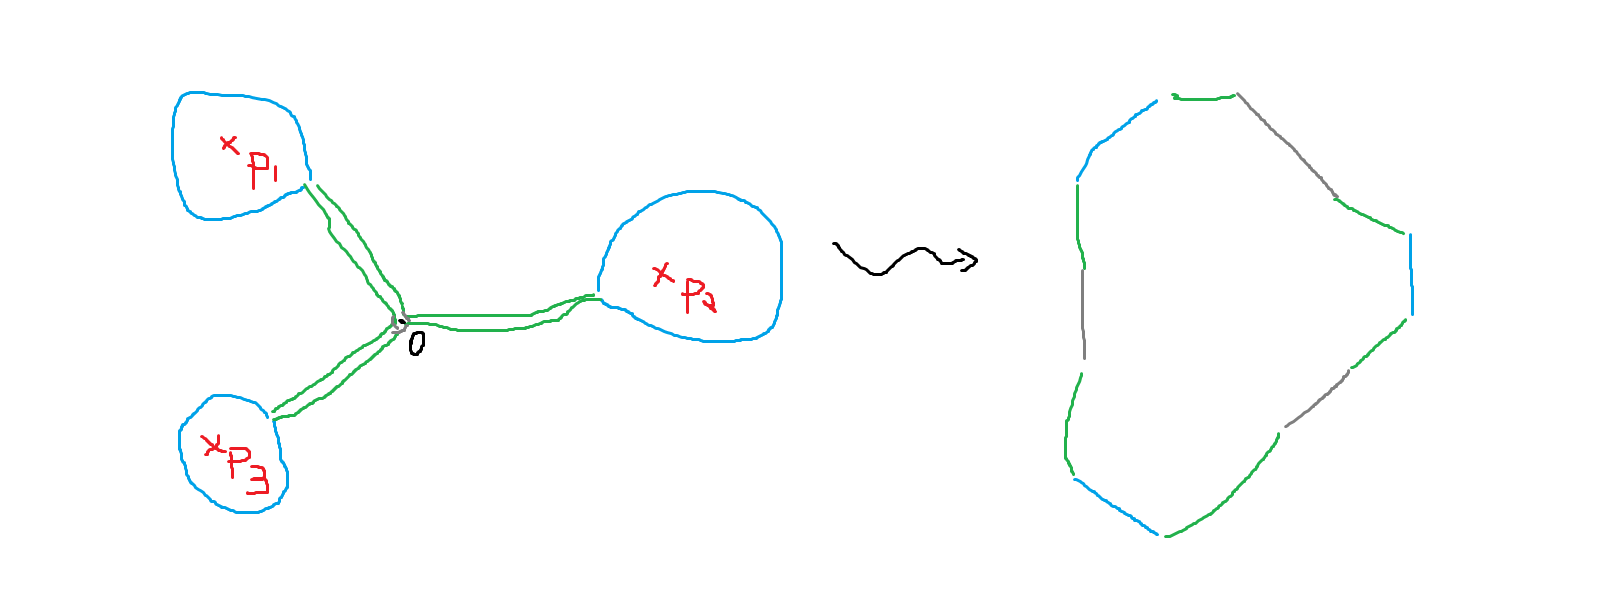
\includegraphics[width=\linewidth]{euler}
\end{figure}

This figure exemplifies a way to map the sphere to $V$ in a way that surrounds every critical point. This map has three parts: The blue part, which surrounds each critical point, and the green part, which connects each critical point to a point (which we called 0) which is not critical. Now, there is a blue and a green part for each critical point, and we need to make sure that each critical point has their own parts, disjoint from everyone else's. Then, in the spaces between the green parts, we have a gray part, which is constant equal to zero. This is important.

First of all, note that this `sphere' can be homotoped to the sphere of radius $R$ without passing by any zeroes of $X$. Therefore, to show that $f$ has degree zero is the same as to show that $X$ composed with this map has degree zero.

Now, we compute the degree of $X$ composed with this map, call this composition $g$. Note that $g$ is constant on the gray parts, always equal to $X_0$.

Pick a representative $\omega$ of the 1-class of the cohomology of $S^1$, and set $\eta = X^* \omega$. Since $X$ is constant on the gray parts, it is clear that $\eta$ is null on them. Therefore, since the blue-green parts are disjoint, we can decompose $\eta = \eta_1 + \eta_2 + \dots$, each $\eta_i$ corresponding to each blue-green part, i.e. one $\eta_i$ for each critical point. Now it suffices to show that $[\eta_i]$ equals the degree of $p_i$.

Note that $\eta_i$ can be built in a similar way to $\eta$, except that we only consider the blue ball around $p_i$ and its corresponding tube. All the other blue and green parts are set to zero instead. Now, this new sphere can be homotoped to the blue sphere around $p_1$ without passing by any critical points of $X$, and therefore the class of $\eta_i$ is the degree of $p_i$, \emph{by definition}! This completes the proof of the lemma, and hence the solution of the exercise.
\end{sol}

\begin{ex}
Let $M$ be a manifold, $S$ a proper oriented submanifold, $\nu$ an embedded tubular neighborhood of $S$. Let $U$ be a representative of the Thom class of $S$ (in the normal bundle $\cong \nu$). Extend $U$ by zero to the whole manifold. Show that $U$ is a representative of the closed Poincaré dual of $S$. Conclude that you can find representatives of the closed Poincaré dual of $S$ whose support is arbitrarily close to $S$.
\end{ex}

\begin{sol}
To show that $U$ is a representative of the Poincaré dual of $S$, we simply pick a $m-s$ form $\omega$ on $M$ (where $m = \dim M$ and $s = \dim S$) and show that
\[\int_M \omega \wedge U = \int_S \omega.\]

This is easy. Since $U$ has support contained in $\nu$,
\[\int_M \omega \wedge U = \int_\nu \omega \wedge U,\]
and by definition of the Thom class, this is the same as $\int_S \omega$.

To draw the conclusion about support of closed Poincaré duals of $S$, we need to show that there exist tubular neighborhoods of $S$ arbitrarily close to $S$. Given a neighborhood $V$ of $S$, we may apply the tubular neighborhood theorem for $S \subseteq V$ in order to obtain a tubular neighborhood of $S$ contained in $V$. The proof is complete.
\end{sol}

\end{document}